\documentclass[a4paper,11pt]{scrartcl}
\usepackage[utf8]{inputenc}
\usepackage{listings}
\usepackage{array}
\usepackage[pdftex]{graphicx}
\usepackage{fancyhdr}
\usepackage[titletoc,title]{appendix}
\usepackage[pdftex,dvipsnames,table]{xcolor}
\usepackage[pdftex,colorlinks=true]{hyperref}
\usepackage{pdfpages}

% page layout
\textheight=25.5cm
\textwidth=16cm
\oddsidemargin0cm
\topmargin-2cm

% set sectioning count levels
\setcounter{secnumdepth}{3}
\setcounter{tocdepth}{4}

% page style for front page
\pagestyle{fancy}
\fancyhead[L,C,R]{}
\fancyfoot[L,R]{}
\fancyfoot[C]{Copyright LSST:UK Consortium 2017}
\renewcommand{\headrulewidth}{0pt}
\renewcommand{\footrulewidth}{0pt}

% page style for other pages
\fancypagestyle{plain}{%
\fancyhf{}%
\fancyhead[C]{\title}%
\fancyfoot[C]{\thepage}%
\renewcommand{\headrulewidth}{0pt}
\renewcommand{\footrulewidth}{0pt}
\setlength{\parskip}{1em}}

% define the title
\def\title{D3.11.2: Demonstration Software for One Example Catalogue}

% set listings format
\lstset{
  frame=single,
  basicstyle=\normalfont \ttfamily,
  stringstyle=\ttfamily 
}

% verbatim code text
\lstnewenvironment{code}[1][]
{\lstset{#1}}
{}

% the comment box
\newcommand{\comment}[1]{\colorbox{Goldenrod}{\parbox{\textwidth}{\textit{#1}}}}

% the inline code box
\newcommand{\inlinecodebox}[1]{\colorbox{lightgray}{\lstinline|#1|}}

% coloured sectioning headers
\addtokomafont{section}{\color{blue}}
\addtokomafont{subsection}{\color{blue!75}}
\addtokomafont{subsubsection}{\color{blue!50}}
\addtokomafont{paragraph}{\color{blue!40}}

\setlength{\parindent}{0pt}

\begin{document}

% LSST logos
\begin{center}
\begin{tabular}{p{6cm}p{4cm}p{6cm}}

\includegraphics[width=5.5cm]{lsst-uk_consortium_small.png} & & 
\includegraphics[width=5.5cm]{lsst-uk_science_centre_small.png} \\
\end{tabular}
\end{center}

% front page
\thispagestyle{fancy}
\begin{center}
% title goes here
{\Huge\textcolor{Blue}{\textbf{\title}}}\\[2ex]

% define the subject
{\LARGE\textcolor{BrickRed}{WP3.11: Cross-Matching and Astrometry at LSST Depths}}\\

\end{center}

% project description
\begin{table}[ht]
\centering
\renewcommand{\arraystretch}{1.75}
\begin{tabular}{>{\bfseries}p{4.5cm}p{11.5cm}}
Project Acronym & LUSC-B\\
Project Title   & UK Involvement in the Legacy Survey of Space and Time\\
Document Number & LUSC-B-11
\end{tabular}
\end{table}

% versioning
\begin{table}[ht]
\centering
\renewcommand{\arraystretch}{1.75}
\begin{tabular}{|>{\bfseries}p{4.5cm}|p{11.5cm}|}
\hline
Submission date & 7/Jan/2021 \\\hline
Version & 2.0 \\\hline
Status  & Final \\\hline
\parbox{4cm}{Author(s) inc. institutional affiliation} & Tom J. Wilson (Exeter) \\ & Tim Naylor (Exeter) \\ & George Beckett (Edinburgh) \\ & Mike Read (Edinburgh) \\\hline
Reviewer(s) & \parbox{11cm}{\raggedright Bob Mann (UEDIN),\linebreak Raphael Shirley (SOTON)}\\\hline
\end{tabular}\\[2ex]
\end{table}

% dissemination level
\begin{table}[ht]
\centering
\renewcommand{\arraystretch}{1.75}
\begin{tabular}{|p{4.5cm}p{11.5cm}|}
\hline
\multicolumn{2}{|l|}{\textbf{Dissemination level}}\\\hline
Public\\\hline
\end{tabular}
\end{table}

\newpage
\pagestyle{plain}
% version history
\section*{Version History}
\addcontentsline{toc}{section}{Version History}

% versions
% if text is longer than the box, use \parbox environment
\begin{table}[ht]
\centering
\renewcommand{\arraystretch}{1.75}
\begin{tabular}{|p{1.5cm}|p{2.5cm}|p{6.5cm}|p{4.5cm}|}
\hline
\textbf{Version} & \textbf{Date} & \parbox{6.5cm}{\textbf{Comments, Changes, Status}} & \parbox{4.5cm}{\textbf{Authors, Contributors, Reviewers}}\\\hline
1.0  & \parbox{2.5cm}{07/01/21} & \parbox{6.5cm}{First draft for review} & \parbox{4.5cm}{Tom J. Wilson}\\\hline
2.0  & \parbox{2.5cm}{22/02/21} & \parbox{6.5cm}{Update with reviewer comments} & \parbox{4.5cm}{Tom J. Wilson}\\\hline
 & & & \\\hline
 & & & \\\hline
 & & & \\\hline
 & & & \\\hline
\end{tabular}
\end{table}

\newpage
\pagestyle{plain}
% create table of contents, tables, and figures
\renewcommand{\contentsname}{Table of Contents}

\tableofcontents
\listoffigures
\listoftables

\newpage
\pagestyle{plain}
\section{Introduction}
WP3.11 is investigating the astrometry of LSST.
An unprecented parameter space in optical photometric surveys, the depths to which the Rubin Observatory will probe during its 10-year initial survey will challenge data reduction and analysis tools.
We are focusing on the problems surrounding the creation of value-added catalogues: those combining the LSST dataset with external, ancillary catalogues, to improve the science that can be done.
To achieve this, we must identify those sources in common between the two catalogues which are truly one physical object on the sky, for which we have two detections.
These must be, in turn, differentiated from sources which simply happen to appear very close in the sky to one another, but are two independent sources in the sky.
This process of creating a single, composite dataset is the "cross-matching" of the two catalogues.

The challenge for LSST is primarily one of sheer source counts.
Never before has an optical survey reached the expected depths of LSST -- 27th magnitude at its full completeness limit -- and thus never had to cope with the increase in source detection rate that goes along with such sensitivity.
And yet the survey will still be limited to ground-based resolutions, with the atmospheric distortions that "spread" out otherwise point source objects into a larger pool of light on the CCD of the telescope.
When crowding of sources, as we expect for LSST, becomes significant, these "point spread functions" (PSFs) can and will start to overlap one another.
Thus a very bright source can "hide" within its PSF a faint object, which the detection algorithms will fail to include in the final catalogue of objects produced by the "LSST stack".
Unfortunately, the faint source can influence the measured position of the bright source, even if it was not detected, by subtly tugging on the centroid of the bright object during its position determination.

Usually a photometric catalogue records the measured position of a source, and a corresponding uncertainty: the precision with which the algorithms and pipelines were able to pinpoint the determined position.
For LSST, these precisions will be very good, and thus the positions will likely be quoted to high confidence.
Crucially, however, these "tugs" from faint sources, buried within the light of the brighter source, can be larger than the precisions with which sources are pinpointed, and thus the simple questions asked by traditional cross-match algorithms "given the positions and corresponding precisions of these two sources, how likely are they to have the same sky position?" will break down.
It is overcoming this limiting factor, expected to be significant for LSST, that WP3.11 is most interested in.

\section{Demonstration Software}
To enable more robust cross-matches of LSST and other catalogues, including the effects of position perturbation from blended objects, WP3.11 is mainly tasked with the creation of new software to allow for such cross-matches to occur.
These matches will then be hosted on the UKDAC, accessible to users.
Thus, after we had established it was possible to overcome or sidestep a few implementation challenges (see the D3.11.1 report for more details), we began the establishment of the codebase core, on to which the more advanced, and WP-focused, algorithms could be added.

\subsection{Deliverable Name}
\label{sec:deliverable_name}
The formal deliverable for D3.11.2 is titled "Demonstration Software for One Example Catalogue".
This is because, during the proposal phase for this WP, it was envisaged that demonstration code would be written to specifically match an example catalogue pair, the code then moved to run on the DAC and subsequently generalised to allow for any catalogue combinations in D3.11.3.
In practice we thought it would save time to go directly to writing the software for the DAC, skipping the demonstration software.
Thus D3.11.2 should really be "Demonstration of Preliminary Software for DAC Integration".
The software that forms D3.11.2 is an end-to-end complete cross-match code, installable by the end user, featuring documentation, but does not yet have the sophisticated algorithms which are WP3.11’s main task and will be the focus of D3.11.3.


\subsection{Preliminary Software}
The software that delivers D3.11.2 is a full, end-to-end, "many-to-many" cross-match code, capable of accepting two catalogues and producing posterior probabilities of likely matches and non-matches between "islands" -- sources potentially astrometrically correlated with one another and definintely not correlated with any other source -- of sources across the two catalogues.
This limit to two catalogues, but allowing for inclusion of multiple matches simultaneously, is what makes it a "many-to-many" match software.
It accepts the astrometric uncertainty -- the precision with which sources were centroided -- and uses the normalised on-sky separation of two sources to calculate their relative match likelihood.
This simple match assumption -- the natural assumption of most match algorithms, ignoring any other systematic effects which might cause separation between sources, such as proper motions or blending -- and the non-inclusion of any other discriminating information that might be used to distinguish between two competing counterparts for a source mean that this implementation is currently a "naive Bayes" cross-match.
However, these assumptions hold for a large number of previous generation photometric catalogues, and even in its half-finished state the cross-match codebase provides useful functionality.

\section{Deliverables}
The main deliverables for this work, being software development, are available online.
As per the Project Management Plan, software development should be maintained in a version control repository.
The main codebase is therefore located at \href{https://github.com/Onoddil/macauff/tree/7891efc9e5edc30febb2d3bcfdb14e97252493d0}{https://github.com/Onoddil/macauff}.
It features a full test suite for validation, as well as functionality to generate test data to input into the cross-match algorithm for end-to-end verification.
The folder structure is as follows.
\begin{itemize}
	\item Top-level files.
	\begin{itemize}
		\item CHANGES.rst: changelog file, itemising the updates to the codebase.
		\item LICENSE and README.md: details of licensing of codebase, and a top-level overview description of the software.
		\item MANIFEST.in, pyproject.toml, and setup.cfg: minor files that aid with the setup and installation of the Python package.
		\item python-package.yaml: within the \texttt{.github/workflow} folder, this details the \texttt{GitHub} virtual environment setup and the running of the test suite.
		\item setup.py: main installation file for the Python package, which describes the various dependencies for installing the package, and controls the compiling of \texttt{fortran} code.
		\item tox.ini: configuration file describing setup of the \texttt{tox} environment for test purposes.
	\end{itemize}
	\item Documentation files, \texttt{docs/}.
	\begin{itemize}
		\item conf.py: configuration file, for Python automated creation of documentation.
		\item *.rst: files containing the raw text that makes up the documentation of the codebase.
	\end{itemize}
	\item Code files, \texttt{macauff/}.
	\begin{itemize}
		\item \_\_init\_\_.py: File used during the installation process, indicating which files and functions should be importable.
		\item counterpart\_pairing*: Python and Fortran code (\texttt{.py} and \texttt{\_fortran.f90} respectively) to run the cross-match assignment functionality and calculate cross-match probabilities.
		\item group\_sources*: Python and Fortran code used in the generation of ``islands'' of potential counterparts, independent of other sources in the respective catalogues.
		\item make\_set\_list.py: Python script used in group\_sources.py to derive ``sets'' of source overlaps on astrometric considerations, based on lists of sources near to each object.
		\item matching.py: Python code handling the overall cross-match process.
		\item misc\_functions*: Python and Fortran code that is used in multiple places throughout the cross-match process, and hence cannot be kept within any single script.
		\item perturbation\_auf.py: Python code to handle the creation of ``dummy'' arrays for the perturbation component of the Astrometric Uncertainty Function. Main algorithms currently not implemented, and included for future backwards compatibility.
		\item photometric\_likelihood.py: Python code to handle the creation of source match likelihoods on photometric grounds. Also currently not implemented for the most part, and featuring backwards compatible code.
		\item shared\_library.f90: Similar to misc\_functions, contains subroutines that are needed across other Fortran modules, and are therefore accessible from those other files.
		\item Test files, \texttt{tests/}.
		\begin{itemize}
			\item \_\_init\_\_.py: same as in the parent folder.
			\item test\_*.py: Unit test scripts, one per Python script in the folder above, to ensure consistency and accuracy of the main codebase.
			\item Data files, \texttt{data/}.
			\begin{itemize}
				\item *.txt: example files of the configuration files used in the cross-match process.
			\end{itemize}
		\end{itemize}
	\end{itemize}
\end{itemize}

In addition, to aid in the review, preliminary documentation -- guides to installation and getting started with the codebase -- is available at \href{https://onoddil.github.io/macauff/}{https://onoddil.github.io/macauff/}.
This documentation, formed from the raw files in \texttt{macauff/docs} in the repository, is structured as follows.

\begin{itemize}
	\item Homepage: brief description of module and links to various starting pages.
	\item Installation: details the installation process of the module, its dependencies, and how to run the test suite to ensure successful installation.
	\item Quick Start: description of how to begin working with the package, describing the necessary files to run a cross-match, and giving examples of how to run matches between two catalogues.
	\item Inputs: more in-depth descriptions of each parameter that should be specified in the input configuration files used in the cross-match process.
	\item Documentation: collection of available functions within both the Python and Fortran code in the codebase, describing the inputs and outputs from each function or subroutine in detail.
\end{itemize}

\section{Future Work}
The main focus of D3.11.3, now that WP3.11 has an established codebase for its software development aims, is to implement the extended algorithmic aspects of its remit.
First, we must include the algorithmic components that extend the Astrometric Uncertainty Function from the simple assumption that centroiding uncertainties are the only component, and include a prescription for the uncertainty in position that derives from the perturbation of a bright source by a fainter contaminant source within its PSF.
Second, we plan to include an additional improvement to better provide users confident cross-matches: the use of the photometry of the sources to distinguish between true coevality in sources and happenstance astrometry; this can be achieved using the idea that as an ensemble sources of 15th magnitude in one optical bandpass are going to have a roughly 15th magnitude source near to them in a similar optical wavelength, but unlikely to experience a 22nd magnitude source being coeval with them.

In addition, we plan to extend and improve the user documentation, both for the current features and for the additional features to be implemented.
This is crucial to ensure that the codebase is useable by the LSST:UK project after the end of this current work package.

\subsection{Data Access Centre Interactions}
One major aspect of WP3.11, which sits in parallel with the deliverables, is the interactions between the ``Dev'' (WP3.11) and ``DAC'' (WP2.5) teams.
Our significant output is so-called Rubin ``User Generated Products'' -- extra products which use and extend Rubin data.
We therefore require the DAC to host these products such that users can interact with them once we have generated them for a given catalogue-catalogue combination.
The workflow also requires the generation of appropriate input tables for the software, which will take the two input catalogues and reduce them to a canonical format for use in the WP3.11 software.

This interaction between WP2.5 and WP3.11 necessitates the formation of workflow documentation, such that these interactions can continue beyond Phase B and WP3.11.
We are in the process of formalising these interfaces between the DAC team, WP3.11, and the community.
We attach here a draft overview of the in-progress interface document, as the interactions between the DAC and WP3.11 were moved forward to be part of the D3.11.2 deliverable during the rearrangement of the package (see section \ref{sec:deliverable_name} for a brief outline of the change).
Formally this interface document should be a part of the D3.11.3 deliverable, however, and hence the full interface document will be finalised in due course.

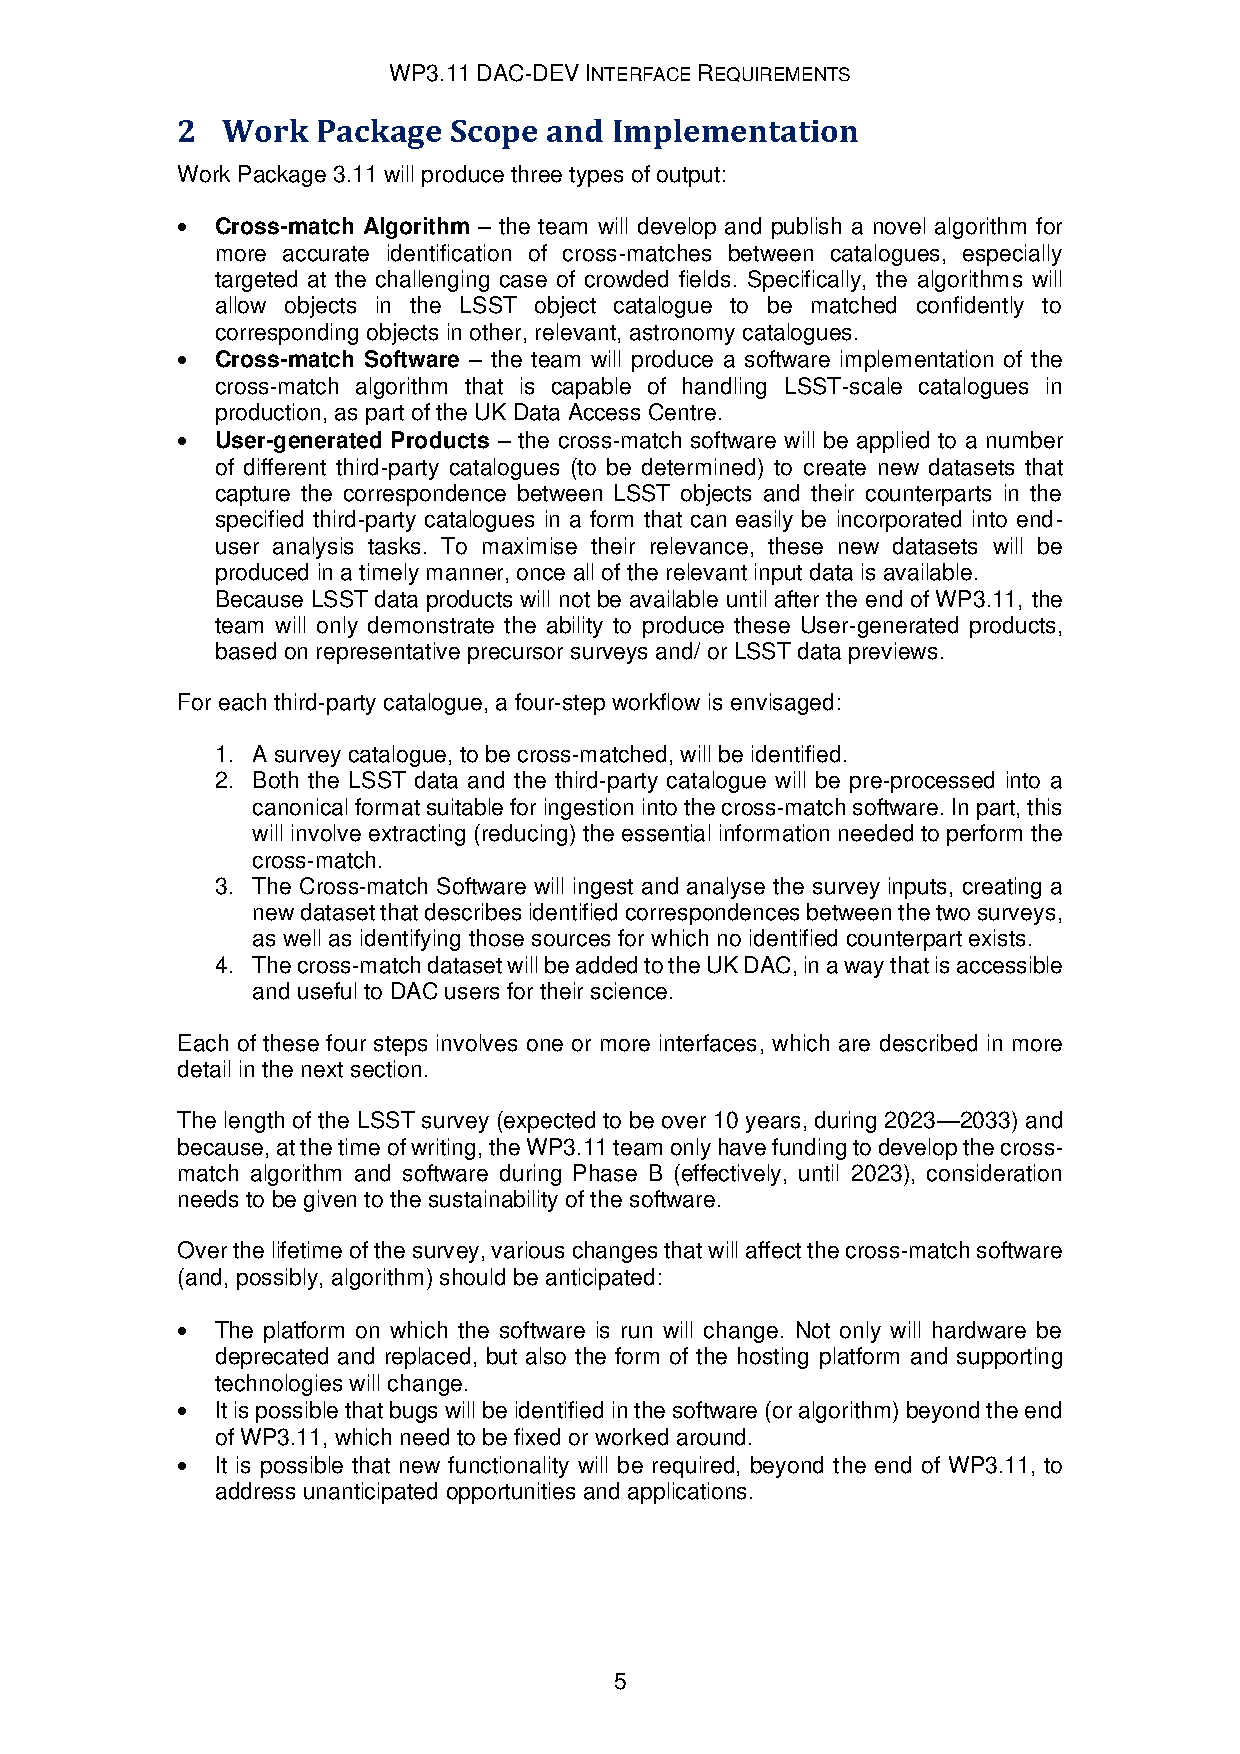
\includepdf[pages=-,offset=0 0]{WP3-11_DAC-DEV_interface_definition.pdf}

\end{document}
